%%%%%%%%%%%%%%%%%%%%%%%%%%%%%%%%%%%%%%%%%
% Short Sectioned Assignment
% LaTeX Template
% Version 1.0 (5/5/12)
%
% This template has been downloaded from:
% http://www.LaTeXTemplates.com
%
% Original author:
% Frits Wenneker (http://www.howtotex.com)
%
% License:
% CC BY-NC-SA 3.0 (http://creativecommons.org/licenses/by-nc-sa/3.0/)
%
%%%%%%%%%%%%%%%%%%%%%%%%%%%%%%%%%%%%%%%%%

%----------------------------------------------------------------------------------------
%	PACKAGES AND OTHER DOCUMENT CONFIGURATIONS
%----------------------------------------------------------------------------------------

\documentclass[paper=a4, fontsize=11pt]{scrartcl} % A4 paper and 11pt font size
\usepackage{amsmath,amsfonts,graphicx}
\usepackage{lastpage}	% Required to determine the last page for the footer
\usepackage{booktabs}
%\usepackage{algpseudocode}
\usepackage{tikz}
\usepackage{algorithm}
\usepackage{algorithmicx}
\usepackage{algpseudocode}
\usepackage[top=2cm, bottom=2cm, left=2cm, right=2cm]{geometry}

\usepackage{listings}
\usepackage{color}
\usepackage{xcolor}
\definecolor{dkgreen}{rgb}{0,0.6,0}
\definecolor{gray}{rgb}{0.5,0.5,0.5}
\definecolor{mauve}{rgb}{0.58,0,0.82}
\lstset{frame=tb,
     %language=Java,
     aboveskip=3mm,
     belowskip=3mm,
     showstringspaces=false,
     columns=flexible,
     basicstyle = \ttfamily\small,
     numbers=none,
     numberstyle=\tiny\color{gray},
     keywordstyle=\color{blue},
     commentstyle=\color{dkgreen},
     stringstyle=\color{mauve},
     breaklines=true,
     breakatwhitespace=true,
     tabsize=3
}

%\usepackage[]{algorithm2e}

\usepackage[T1]{fontenc} % Use 8-bit encoding that has 256 glyphs
\usepackage{fourier} % Use the Adobe Utopia font for the document - comment this line to return to the LaTeX default
\usepackage[english]{babel} % English language/hyphenation
\usepackage{amsmath,amsfonts,amsthm} % Math packages

\usepackage{lipsum} % Used for inserting dummy 'Lorem ipsum' text into the template

\usepackage{sectsty} % Allows customizing section commands
\allsectionsfont{\centering \normalfont\scshape} % Make all sections centered, the default font and small caps

\usepackage{fancyhdr} % Custom headers and footers
    \pagestyle{fancyplain} % Makes all pages in the document conform to the custom headers and footers
    \fancyhead[L]{\textsc{COMP90038 Assignment 2}}
    \fancyhead[R]{\textsc{Student Number: 955986 }} % No page header - if you want one, create it in the same way as the footers below
    \fancyfoot[L]{} % Empty left footer
    \fancyfoot[C]{} % Empty center footer
    \fancyfoot[R]{\textsc{Page} \thepage \textsc{ of} \pageref{LastPage}} % Page numbering for right footer
    \renewcommand{\headrulewidth}{0pt} % Remove header underlines
    \renewcommand{\footrulewidth}{0pt} % Remove footer underlines
    \setlength{\headheight}{13.6pt} % Customize the height of the header

\numberwithin{equation}{section} % Number equations within sections (i.e. 1.1, 1.2, 2.1, 2.2 instead of 1, 2, 3, 4)
\numberwithin{figure}{section} % Number figures within sections (i.e. 1.1, 1.2, 2.1, 2.2 instead of 1, 2, 3, 4)
\numberwithin{table}{section} % Number tables within sections (i.e. 1.1, 1.2, 2.1, 2.2 instead of 1, 2, 3, 4)

\setlength\parindent{0pt} % Removes all indentation from paragraphs - comment this line for an assignment with lots of text

%----------------------------------------------------------------------------------------
%	TITLE SECTION
%----------------------------------------------------------------------------------------

\newcommand{\horrule}[1]{\rule{\linewidth}{#1}} % Create horizontal rule command with 1 argument of height

\title{	
\normalfont \normalsize 
\textsc{The University of Melbourne } \\ [25pt] % Your university, school and/or department name(s)
\horrule{0.5pt} \\[0.4cm] % Thin top horizontal rule
\huge COMP90038  Algorithms and Complexity SM2, 2018
Assignment 2 \\ % The assignment title
\horrule{2pt} \\[0.5cm] % Thick bottom horizontal rule
}

\author{Peiyong Wang $\,$ 955986 } % Your name

\date{\normalsize\today} % Today's date or a custom date

\begin{document}

\maketitle % Print the title
\thispagestyle{empty}%no head or foot on the first page


\section{Problem One}
See Figure 1.1.

\begin{figure}[htbp!]
		\centering
		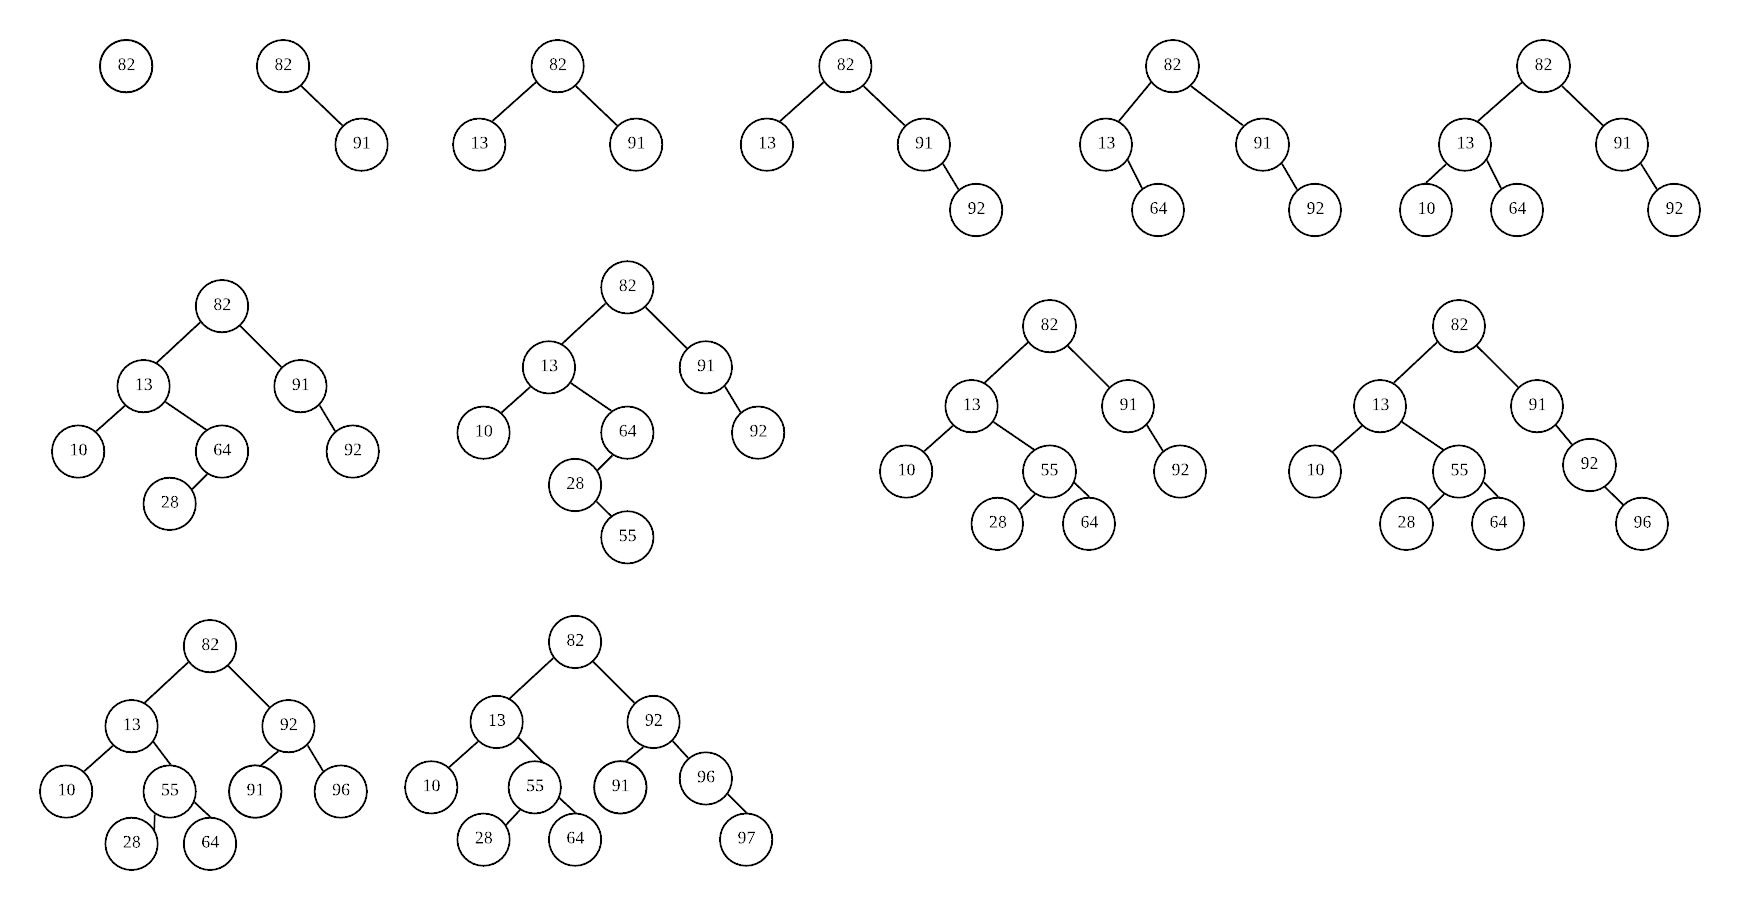
\includegraphics[width=0.9\textwidth]{f1.png}
		\caption{Answer for Problem 1}%\label{book}
		\vspace{-1em}
\end{figure}


\section{Problem Two}
\paragraph{a}

See Algorithm 1.

The time complexity of Algorithm 1 should be O($min(mlog_2m+nlog_2m, mlog_2n+nlog_2n)$), where m and n are the size of X and Y, respectively.
\begin{algorithm}
	\caption{Find intersections of two sets with sorting}
	\begin{algorithmic}[1]
		\Require Two sets of integers X and Y
		\Function{FindSetIntersection}{$X, Y$}
            \State I = [] \Comment initialize the intersection as empty
            \If{$X.size \geq Y.size$}
            \State smallArray = \Call{MergeSort}{Y}
            \State largeArray = X
            \Else
            \State smallArray = \Call{MergeSort}{X}
            \State largeArray = Y

            \EndIf

            \For{every element c in largeArray}
            \State searchResult = \Call{BinSearch}{smallArray, smallArray.size,c}
            \State \Comment Call the BinSearch algorithm from lecture 10.
            \If{searchResult is not -1} \Comment If c exists in smallArray
            \State I.append(c) \Comment copy c to I


            \EndIf


            \EndFor
            \State \Return{ I}

            
			
		\EndFunction
	\end{algorithmic}

\end{algorithm}

\paragraph{b}
See Algorithm 2.

The time complexity of Algorithm 2 should be $ O(m+n)$, where m and n are the size of X and Y, respectively.

\begin{algorithm}
	\caption{Find intersections of two sets with hashing}
	\begin{algorithmic}[1]
		\Require Two sets of integers X and Y
		\Function{FindSetIntersection}{$X, Y$}
            \State I = [] \Comment initialize the intersection as empty
            \State S = \Call{HashSet}{}()\Comment initialize an empty hash set
            \For{every x in X }
            \State S.add(x)

            \EndFor
            \For{every y in Y }
            \If{S.contains(y)}
            \State I.append(y)

            \EndIf

            \EndFor
            \State \Return{ I}

            
			
		\EndFunction
	\end{algorithmic}

\end{algorithm}

\section{Problem Three}
See Algorithm 3. 

For a node i with children [1,2,3,...,n], of which childern 1 needs the most time to pass the message to all its childern and childern n needs the least time to pass the message to all its childern. So we can get through mathematical induction that the time that node i needs to pass the message to all its childern T(i) = n + max(T(n), T(n-1)-1, T(n-2)-2,...,T(1)-(n-1))

Time complexity is O($n^2logn$).

\begin{algorithm}
	\caption{ compute the minimumnumber of days required for the decision to be disclosed to all employee}
	\begin{algorithmic}[1]
		\Require Employee tree C[][]
		\Function{MinDays}{C[][]}
            
            \State \Return{\Call{MinDaysForEmployeeI}{C[][],0}}

            
			
        \EndFunction
        \Function{MinDaysForEmployeeI}{C[][], i}
        \If{C[i][0] is 0}
        \State \Return{0}
        \EndIf
        \State childNodes = []\Comment initialize an empty to store child nodes of i
        \If{C[i][0] is not 0 }
        
        \State m = 1
        \While{C[i][m] is not -1}
        \State childNodes.append(C[i][m])
        \State  m = m+1

        \EndWhile
        \EndIf
        \State days = [\Call{MinDaysForEmployeeI}{C[][], x} for x in childNodes]
        \State days = \Call{QuickSort}{days}
        \For{j from 0 to days.length - 1}
        \State days[j] = days[j] - j

        \EndFor
        \State dayI = C[i][0] + \Call{Max}{days} \Comment function Max() has time complexity O($\frac{3n}{2}$)
        \State \Return{dayI}
        
        
        

        \EndFunction
	\end{algorithmic}

\end{algorithm}

\section{Problem Four}
\paragraph{a} See Algorithm 4. The time complexity should be O(n), where n is the length of input array.


\begin{algorithm}
	\caption{Find the nearest larger element}
	\begin{algorithmic}[1]
		\Require An array of integers A[]
		\Function{NextLarger}{A[]}
            \State res = list(n, -1)\Comment initialize a list of length n and all of its elements are -1
            \State monoStack = stack()\Comment initialize an empty stack
            \For{i from to A.size - 1}
            \While{monoStack is not empty AND A[monoStack.top]<A[i]}
            \State res[monoStack.top] = i
            \State monoStack.pop

            \EndWhile
            \State monoStack.push(i)

            \EndFor
            \State \Return{res}


            
			
		\EndFunction
	\end{algorithmic}

\end{algorithm}

\paragraph{b}
See Algorithm 5. The time complexity should be O($2nlog_2n+n$) = O($nlogn$)

\begin{algorithm}
	\caption{For each of the elementA[i], find the minimumA[j] so thatA[j]> A[i] andj > i}
	\begin{algorithmic}[1]
		\Require An array of integers A[]
		\Function{NextSmallestLarger}{A[]}
            \State res = list(n, -1)\Comment initialize a list of length n and all of its elements are -1
            \State B = [][] \Comment initialize B as a 2-D list
            \State B = [[A[i],i] for i from 0 to A.length -1] \Comment store A[i] and i, B = [[A[0],0],\dots,[A[n-1], n-1]]
            \State \Call{MergeSort}{B[$\cdot$][0]}\Comment sort B according to values from A
            \State \Call{MinHeapArray}{B[$\cdot$][0]} \Comment Turn B[$\cdot$][0] into a min heap stored in an array, original index sift with values from A
            \State listOfJ = B[$\cdot$][1] \Comment original index after sorted with elements from A


            \State monoStack = stack()\Comment initialize an empty stack
            
            \For{j from 0 to n-1}
            \While{monoStack is not empty AND B[monoStack.top][1] < B[j][1] AND B[monoStack.top][0] < B[j][0]}
            \State res[B[monoStack.top][1]] = listOfJ[j]
            \State monoStack.pop

            \EndWhile
            \State monoStack.push(j)

            \EndFor
            \State \Return{res}


            
			
		\EndFunction
	\end{algorithmic}

\end{algorithm}














\end{document}



%\begin{align} 
%\begin{split}
%(x+y)^3 	&= (x+y)^2(x+y)\\
%&=(x^2+2xy+y^2)(x+y)\\
%&=(x^3+2x^2y+xy^2) + (x^2y+2xy^2+y^3)\\
%&=x^3+3x^2y+3xy^2+y^3
%\end{split}					
%\end{align}





%\begin{tabbing}
%\hspace*{.25in} \= \hspace*{.25in} \= \hspace*{.25in} \= \hspace*{.25in} \= \hspace*{.25in} \=\kill
%\>$Euclid(m,n)=$ \\
%\>\> {\bf while} n$ \neq $ 0 \\
%\>\>\> r $ \leftarrow $ $m$ mod $n$  \\
%\>\>\>  m $\leftarrow$n\\
%\>\>{\bf return} m 
%\end{tabbing}

%Python code:
%\begin{lstlisting}[language = python]
%def gcd(m,n):
%	while n != 0:
%		r = m % n
%		m = n
%		n = r
%	return m
%\end{lstlisting}


%\paragraph{Heading on level 4 (paragraph)}




%\begin{tabbing}
%	\hspace*{.25in} \= \hspace*{.25in} \= \hspace*{.25in} \= \hspace*{.25in} \= \hspace*{.25in} \=\kill
%	{\bf function} find (A,x,n)\\
%	\> j $\leftarrow$ 0\\
%	\> {\bf while} j < n\\
%	\>\> {\bf if} A[j]=x\\
%	\>\>\>  {\bf return} j  \\
%	\>\> j $\leftarrow$ j+1\\
%	\> {\bf return} -1
%\end{tabbing}


%\begin{figure}[htbp!]
%		\centering
%		\includegraphics[width=0.6\textwidth]{lec26.png}
%		\caption{Linked List}%\label{book}
%		\vspace{-1em}
%\end{figure}






%\begin{align}
%A = 
%\begin{bmatrix}
%A_{11} & A_{21} \\
%A_{21} & A_{22}
%\end{bmatrix}
%\end{align}



%\begin{algorithm}
 %       \caption{Count the number of occurrences of a certain integer $x$ in an array $A[]$}
  %      \begin{algorithmic}[1] %每行显示行号
   %         \Require  $Array$ A[],$Length\;of\;the\;array$ n, $Integer$ x
    %        \Ensure   Number of occurrence of integer x  
     %       \Function {NumberCount}{$A[], x,n$}
      %      
       %     	\State $firstApperence \gets $\Call{FirstOccurrenceSearch}{$A[]$,0,$n-1$,$x$,$n$}
            	
        %    	\If{$firstApperence=-1$}
         %   	\State \Return $firstApperence$
          %  	\EndIf
            	
           % 	\State $lastApperence\gets$ \Call{LastOccurrenceSearch}{$A[],firstApperence,n-1,x,n$}
            %	\State \Return $lastApperence-firstApperence+1$
            	
                %\State $result \gets 0$
                
                %\If {$high \geqslant low$}
                    %\State $mid \gets (high + low) // 2$   \#"//" means integer division
                    %\State $result \gets result +$ \Call{MergerSort}{$Array, left, middle$}
                    %\State $result \gets result +$ \Call{MergerSort}{$Array, middle, right$}
                    %\State $result \gets result +$ \Call{Merger}{$Array,left,middle,right$}
                %\EndIf
                %\If {$mid = 0 \, OR x > A[mid-1]$}
                %	\State \Return $mid$
                %\Else 
                %	\If {$x>A[mid]$}
                %		\State \Return 
                
                 %\Return{$result$}
            %\EndFunction
           %\State
            %\Function{FirstOccurrenceSearch}{$A[],low, high,x,n$}
            
      %      \If{$high \geqslant low$}
      %      \State $mid\gets(low + high)//2$ \Comment "//" means integer division
      %      \EndIf
      %      \If{$\{mid = 0 \; OR\;  x>A[mid-1]\}\; AND\; \{A[mid]=x\}$} 
      %      \State \Return $mid$
      %      \Else
      %      	\If{$x>A[mid]$}
      %      	\State \Return \Call{FirstOccurrenceSearch}{$A[],mid+1,high,x,n$}
      %      	\Else
      %      	\State \Return \Call{FirstOccurrenceSearch}{$A[],low,mid-1,x,n$}
      %      	\EndIf
      %      \EndIf
      %      \State \Return -1
      %      
      %      \EndFunction
      %      
      %      \State
      %      \Function{LastOccurrenceSearch}{$A[],low,high,x,n$}
      %      
      %      \If{$high \geqslant low$}
      %      \State $mid\gets(low + high)//2$ \Comment "//" means integer division
      %      \EndIf
      %      \If{$\{mid = n-1 \; OR\;  x<A[mid-1]\}\; AND\; \{A[mid]=x\}$} 
      %      \State \Return $mid$
      %     \Else
       %     	\If{$x<A[mid]$}
        %    	\State \Return \Call{LastOccurrenceSearch}{$A[],low, mid-1, x,n$}
         %   	\Else
          %  	\State \Return \Call{LastOccurrenceSearch}{$A[],mid+1, high,x,n$}
           % 	\EndIf
            %\EndIf
            %\State \Return -1
            
            

           % \EndFunction
            
            %\Function{Merger}{$Array, left, middle, right$}
             %   \State $i\gets left$
              %  \State $j\gets middle$
               % \State $k\gets 0$
               % \State $result \gets 0$
               % \While{$i<middle$ \textbf{and} $j<right$}
                %    \If{$Array[i]<Array[j]$}
                 %       \State $B[k++]\gets Array[i++]$
                  %  \Else
                   %     \State $B[k++] \gets Array[j++]$
                    %    \State $result \gets result + (middle - i)$
                    %\EndIf
                %\EndWhile
                %\While{$i<middle$}
                %    \State $B[k++] \gets Array[i++]$
                %\EndWhile
                %\While{$j<right$}
                %    \State $B[k++] \gets Array[j++]$
                %\EndWhile
                %\For{$i = 0 \to k-1$}
                %    \State $Array[left + i] \gets B[i]$
                %\EndFor
                %\State \Return{$result$}
            %\EndFunction
      %  \end{algorithmic}
    %\end{algorithm}


    %\begin{figure}[htbp]
     %   \centering
        
      %  \begin{tikzpicture}
       %     [level distance=1.3cm,
%        level 1/.style={sibling distance=8cm, level distance=0.8cm},
%       level 2/.style={sibling distance=4cm, level distance=0.8cm},
%        level 3/.style={sibling distance=2cm, level distance=0.8cm},
%        level 4/.style={sibling distance=1cm, level distance=0.8cm}]
%        \node {A}
%       child{node{B}
%            child{node{\color{blue}D}
%%                child{node{H}
 %                   child{node{\color{red}1}}
%                    child{node{2}}}
%                child{node{I}
%                    child{node{3}}
%                    child{node{4}}}}
%            child{node{E}
%                child{node{\color{blue}J}
%                   child{node{\color{red}5}}
%                    child{node{6}}}
%                child{node{\color{blue}K}
%                    child{node{7}}
%                    child{node{\color{red}8}}}}}
%        child{node{C}
%            child{node{F}
%                child{node{\color{blue}L}
%                    child{node{9}}
%                    child{node{\color{red}10}}}
%                child{node{\color{blue}M}
%                    child{node{\color{red}11}}
%                    child{node{12}}}}
%            child{node{\color{blue}G}
%                child{node{N}
%                    child{node{13}}
%                    child{node{14}}}
%                child{node{O}
%                    child{node{\color{red}15}}
%                    child{node{16}}}}}
%        ;
%        
%        \end{tikzpicture}
%        \caption{Adaptive tree walk protocol for solving contention. Red digits are stations which are ready,
%        blue characters are the nodes where the contention is resolved.}
%    \end{figure}


